\question[6]
Ermittle mit dem Algorithmus von Dijkstra die kürzesten Wege von Knoten a zu allen anderen
Knoten.  Notiere die Reihenfolge der endgültig markierten Knoten.
Notiere für jeden Knoten die Reihenfolge der Werte, mit denen er markiert wird.

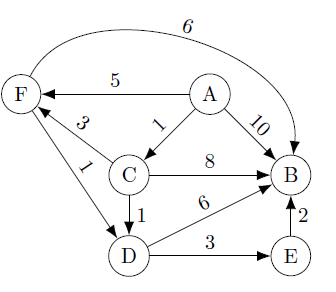
\includegraphics[height=4cm]{\pfad/Graphen/Aufgaben/dijkstra_03/dijkstra_03.png}
\begin{solutionbox}{5cm}
\begin{lstlisting}
Reihenfolge der endgültigen Markierungen: a c d f e b
a : 0
b : inf 10 9 8 7
c : inf 1
d : inf 2
e : inf 5
f : inf 5 4
\end{lstlisting}
\end{solutionbox}
